%This file derives from the ACL template: https://github.com/acl-org/acl-style-files. Adaptation in French: Simon Gabay
%update: Humanistica 2024, Simon Gabay

% This must be in the first 5 lines to tell arXiv to use pdfLaTeX, which is strongly recommended.
%\pdfoutput=1
% In particular, the hyperref package requires pdfLaTeX in order to break URLs across lines.

\documentclass[11pt,french]{article}
\usepackage[utf8]{inputenc}
% Remove the "review" option to generate the final version.
\usepackage{humanistica}

%\usepackage[review]{humanistica}
\usepackage{stfloats}
\usepackage{afterpage}
\usepackage{fancyhdr}
% Set up the fancyhdr package
\pagestyle{fancy}
\fancyhf{} % Clear all header and footer fields
\renewcommand{\headrulewidth}{0pt}
% Add custom header and footer
\fancyfoot[R]{ \thepage}


% Standard package includes
\usepackage{times}
\usepackage{latexsym}
\usepackage{booktabs}

%here are the packages added for my own reading confort they'll be deleted in the final version
\usepackage[parfill]{parskip} % paragraph managing 
\setlength{\parskip}{10pt} %space between the paragraphs
\usepackage{xcolor} %underlines the problematic writting
\usepackage{tabularx}
\usepackage{graphicx}
\usepackage{placeins} % For \FloatBarrier
\usepackage{geometry}
\usepackage{array} % For advanced column specifications
\usepackage{amsmath}
\usepackage{multirow}
\usepackage{makecell}  
\newcolumntype{P}[1]{>{\arraybackslash}p{#1}<{\rule{0pt}{3ex}}}
\usepackage{enumitem}% customize bullet point

% For proper rendering and hyphenation of words containing Latin characters (including in bib files)
\usepackage[T1]{fontenc}
% For Vietnamese characters
% \usepackage[T5]{fontenc}
% See https://www.latex-project.org/help/documentation/encguide.pdf for other character sets

% This assumes your files are encoded as UTF8
\usepackage[utf8]{inputenc}

% This is not strictly necessary, and may be commented out,
% but it will improve the layout of the manuscript,
% and will typically save some space.
\usepackage{microtype}

%Translate to French
\usepackage{babel}
\def\frenchtablename{Tableau}

% If the title and author information does not fit in the area allocated, uncomment the following
%
%\setlength\titlebox{<dim>}
%
% and set <dim> to something 5cm or larger.

\title{Vers une exégèse digitale : OCR et topic modeling \\ Étude du \textit{Commentaire de la Première épître à Timothée} \\ de Lambert Daneau (1530-1595)}

% Author information can be set in various styles:
% For several authors from the same institution:
% \author{Author 1 \and ... \and Author n \\
%         Address line \\ ... \\ Address line}
% if the names do not fit well on one line use
%         Author 1 \\ {\bf Author 2} \\ ... \\ {\bf Author n} \\
% For authors from different institutions:
% \author{Author 1 \\ Address line \\  ... \\ Address line
%         \And  ... \And
%         Author n \\ Address line \\ ... \\ Address line}
% To start a seperate ``row'' of authors use \AND, as in
% \author{Author 1 \\ Address line \\  ... \\ Address line
%         \AND
%         Author 2 \\ Address line \\ ... \\ Address line \And
%         Author 3 \\ Address line \\ ... \\ Address line}

\author{Floriane GOY \\
  UNIGE / Institut d'Histoire de la Réformation \\}
  %Affiliation / Adresse ligne 2 \\
 % Affiliation / Adresse ligne 3 \\
%\texttt{email@domaine} \\\And
 % Second Author \\
  %Affiliation / Adresse ligne 1 \\
 % Affiliation / Adresse ligne 2 \\
 % Affiliation / Adresse ligne 3 \\
%  \texttt{email@domaine} \\}

\begin{document}
\maketitle
\begin{abstract}
Mettre un résumé de (une phrase chaque point):
- ce sur quoi tu travail (Paul, etc.)
- Ce que tu as fait (acquisition OCR, extraction lematisation et topic modelling)
- Quels sont tes résultats
Max:150 mots\par

\end{abstract}

\section{Introduction}
%Décrire le problème en terme de sciences humaines pure
%Sur la Renaissance
-Rennaissance et Reforme 
-le latin de Lambert Daneau et des exegetes du XVIe
-Pourquoi une approche numérique, avantage et inconvéniant de la methode

\subsection{ la Renaissance et le commentaire exégétique au XVIe siècle} %corrigé
L'invention de l'imprimerie est un facteur déterminant pour comprendre les changements culturels qui caractérisent la Renaissance et définissent cette période de transition entre la fin du Moyen Âge et le début l'Époque Moderne. Or, le premier texte imprimé ne pouvait être que la Bible, l'ouvrage au centre des préoccupations des chrétiens depuis plus de mille ans. Au milieu du XV\textsuperscript{e} siècle, l'impression la fameuse Bible de Gutenberg  dans la ville de Mayence signe ainsi l'acte de naissance de cette nouvelle pratique. Mais le développement de cette technologie exacerbe rapidement une série de problématiques, auparavant largement restreintes par les conditions de production des copies manuscrites. Quels textes diffuse-t-on, qui a le droit de les distribuer ou de les imprimer, comment garder le contrôle sur la reproduction d'un document et sur son contenu? Ces interrogations sont centrales pour la société de la fin du Moyen Âge dont une partie de l'élite s'est consacrée jusqu'à lors à la lecture et l'interprétation des textes. Parmi les disciplines de l'herméneutique, la Théologie s'est constituées comme la première des sciences durant Moyen Âge et son étude offre un prestige tout particulier à ses praticiens. Les travaux des théologiens se concentrent ainsi sur la transmission et l'analyse des enseignements de la Bible dont ces derniers considèrent la doctrine comme porteuse d'une vérité unique incarnée dans le Verbe divin ainsi que dans sa langue : le latin.\par 
Dans le monde intellectuel du XVe siècle largement dominé par le latin, un événement historique, \textit{a priori} militaire, revêt également une place non négligeable dans l'histoire des textes. En 1453, la ville de Constantinople est définitivement prise par les armées turques du Sultan Mehmet II. Tandis que la cité grecque devient la capitale de l'empire ottoman, les érudits chrétiens cherchent refuge dans les villes italiennes, leurs anciens partenaires commerciaux. Sur la route de l'exile, ils apportent avec eux de précieux manuscrits byzantins ainsi qu'une connaissance intime du grec ancien dont l'empire d'orient n'a jamais perdu la pratique contrairement à son voisin d'occident. L'arrivée de cette culture hellénistique, au moment même où l'imprimerie commence à se développer, contribue à diffuser et à perfectionner à l'échelle européenne des méthodologies à l'étude depuis le Trecento et les premières investigations philologiques de Lovato Lovati~(1240-1309) \cite[p.101-104]{reynoldsChapitreIVRenaissance2021}. Au coeur de ces réflexions, se trouve la question de l'authenticité des texte, et de leurs attributions. La problématique est d'autant plus brûlante lorsqu'elle concernent textes sacrés dont l'autorité est fondée sur ces valeurs. En 1440, Lorenzo Valla~(1407–1457) démontre ainsi que la \textit{Donation de Constantin} est un faux et conteste l'authenticité de la correspondance entre Paul et Sénèque. Il commence également à travailler sur la Vulgate en la corrigeant à l'aide d'originaux grec et de texte patristique \cite[p.118]{reynoldsChapitreIVRenaissance2021}. En 1505, Erasme~(1466-1536) imprime les corrections du savant italien et s'appuie sur ces travaux pour mettre au point le \textit{Novum Instrumentum}, l'édition du Nouveau Testament grec. En 1516, la Bible d'Erasme est imprimée, elle devient l'outil par excellence des commentateurs de la Bible, lorsqu'il est question du texte grec. Ce faisant Erasme pérennise la méthodologie développé par Valla et ses confères : l'étude d'un texte doit se fonder autant que possible sur des originaux et non sur des traductions, les Ecritures sont interprétables comme tout autres ouvrage ouvrages selon les mêmes critères logique \cite[p.~126]{reynoldsChapitreIVRenaissance2021}.\par 
Dans le XVI\textsuperscript{e} siècle de Lambert Daneau (1530-1595), la diffusion des nouvelles pratiques philologiques a ainsi des conséquences tout particulièrement sur la pratique de l’interprétation du texte par essence qu’est l’exégèse biblique. Lorsque la Renaissance est considérée dans son interaction avec la Réforme, son étude souligne principalement la transformation du rapport entre l'intellectuel et les Écritures tant sur le plan matériel et que méthodologique.\par
%Sur la théologie de la Renaissance. 
Le XVI\textsuperscript{e} siècle marque ainsi la fin de l'usage unilatéral de la Vulgate médiévale, la Bible écrite par Jérôme aux environs du IV\textsuperscript{e} siècle. L'entreprise de traduction du texte biblique vers les langues vulgaires et le retour à l'étude des versions antérieures du texte rédigées en grec et en hébreu ont fait évoluer la compréhension du corpus biblique. Les commentateurs perçoivent désormais l'hétérogénéité de l'écriture sainte et examinent les différentes strates de sa construction. L'exégèse, si elle s'écrit toujours en latin, repose davantage sur un argumentaire philologique étayé par l'analyse des textes écrits dans langues première de la bible. Dans le cas des épîtres pauliniennes rédigées en grec, cette langue sert tout particulièrement le travail du commentateur. Cette approche du texte biblique à travers ses traductions n'est pas une nouveauté de la Renaissance, ni même de la Réforme, et les exégètes moderne leurs précurseurs médiévaux comme Paul de Burgos (1351-1435) ou Nicolas de Lyre (1270-1349) \cite[p.~239]{dahanExtraitPrefaceBible2017}, mais l'amplification de ce mouvement au XVI\textsuperscript{e} siècle traduit une évolution générale dans la conception de la Bible.\linebreak
Dans le monde catholique, cette prise de conscience de la pluricité du texte sacré est discuté lors du concile de Trente(1546) et aboutit à la publication en 1592 de la Vulgate dite sixto-clémentine dont l'édition fera référence jusqu'au XX\textsuperscript{e} siècle \cite[p.9-10]{dahanVulgateAuXVIe2020}. cherchent ainsi à garantir l'unicité de la parole divine en légiférant s et établir son autorité incontestable approuvée par la hiéarchie du clergé. La situation est encore plus complexe du côté des réformés qui sans abandonner la lecture de la Vulgate traditionnelle , travaillent sur diverses versions du texte. Ces révisions successives du texte biblique prennent désormais le nom de \textit{Biblia sacra emendata} \cite[p.127]{noblesse-rocherRevisionsVulgateDans2020}, des bibles corrigées. Le commentateur réformé donc à  travers une pluralité de textes, il an tête des \textit{Biblia} et se trouve éternellement dans un exercice de traduction du grec ou de l'hébreu vers le latin. Tout en conservant certains acquis de la pensée scolastique, l'exégèse de la Réforme emploie les nouvelles méthodologies développées dans les cercles humanistes.\par
Enfin, il faut souligner la dimension apologétique que prennent les commentaires réformés puisque les exégètes doivent désormais défendre et affirmer les principes de la nouvelle religion \cite{boisson2012apologies}. Avec sa réflexion théologique, le commentateur chercher à transmettre une réflexion politique et morale visant à organiser les domaines de la vie publique comme privée.\par   
\subsection{Les Néo-Latins}
%Sur le latin (de la Renaissance)
Le latin de la Renaissance, de son nom savant Néo-latin est, comme tout idiome au long cours, constitué de différentes strates de lexique accumulé à travers le temps. Peut-être faudrait-il également dire les latins de la Renaissance? Tant il est vrai qu'aux yeux du spécialiste, le latin d'oeuvre comme l'\textit{Africa} de Pétrarque  est lointain de celui des commentateurs bibliques. Les noms de Néo-latin et Mediolatin définissent avant tout une segmentation chronologique et non une réalité linguistique \cite[p.142]{tilgMedievalLatinNeoLatin2015}. \textcolor{red}{expliquer la périodisation}\\
Le latin des théologiens de la première modernité est une langue technique poursuivant un objectif de clarté qui fait appel à un vocabulaire spécialisé. Par voie de conséquence, son utilisateur emploie le langage du latin chrétien ou latin patristique car la tradition a depuis longtemps assimilée ses formulations qui sont celle de la Vulgate de Jérôme et de ses premiers commentateurs. A ce vocabulaire né dans l'antiquité tardive est associé un discours proprement médiéval dans lequel le lexique scolastique est largement majoritaire. Là encore rien d'étonnant, puisque la langue des théologiens et les philosophes des XIII\textsuperscript{e} et XIV\textsuperscript{e} siècles est celle qui a servi de cadre aux réflexion des penseurs de la première modernité (XV\textsuperscript{e}-XVI\textsuperscript{e} siècle) \cite[p.34-37]{blumPhilosophenphilosophieUndSchulphilosophie1998}. Les nouveautés lexicales proviennent majoritairement de calques latins traduisant des concepts grecs, entrés dans la langue avec l'assimilation de la culture hellénistique. Loin des enjeux esthétiques propres aux oeuvres littéraires, le latin de l'exégèse du XVI\textsuperscript{e} siècle ne fait pas l'objet d'une recherche consciente du classicisme. Par bien des aspects, ce néo-latin ecclésiastique est plus proche latin médiéval des ecclésiastiques que du latin littéraire des humanistes.\par
%https://humanistica-helvetica.unifr.ch/fr/introduction/what-is-neolatinism
%Sur le topic modelling
Ces réflexions sur la "qualité" de la langue sont importantes pour le topic modelling qui implique la mise au point d'un modèle de langue pour traiter en les lemmatisant chacun des mots du corpus. Or, en construisant ce modèle sur la base d'un latin ecclésiastique du XVI\textsuperscript{e} siècle, il sera également possible de le tester sur d'autres formes de latin pour comprendre en quoi la variance des lexiques est significative dans le résultat de l'analyse. Est ce que le modèle construit avec l'apport du vocabulaire de Lambert Daneau peut servir à l'étude d'un poème de la même période? Qu'en est-il s'il est question d'un contenu plus similaire comme celui d'autres livres de la Bible? Qu'elle distance y a-t-il entre le vocabulaire employé pour commenter un livre de l'ancien testament comme la Genèse et le texte d'un contenu \textit{a priori} plus proche le serait autre épître de Paul?\\
Ces questions paraissent à première vue liminaire au cadre restreint du projet mais elle lui sont en réalité nécessaires car les résultats de l'analyse permettront de calibrer le modèle en vue de son usage à grande échelle dans les commentaires du corpus pauliniens du XVI\textsuperscript{e} siècle.\\ Dans le cadre du présent travail, la comparaison linguistique s'appuiera uniquement sur des textes appartenant à la période du neolatin (1430-1800) mais il est évident que dans une étude plus large, l'inclusion dans le teste des textes en mediolatin seraient souhaitables. d'interroger la continuité linguistique entre la fin du Moyen-Age et le début de l'époque moderne.\par 

\section{Problématique}

le travail sur le latin du 16e
décrire les objectif : outil pour faire ressortir les thèmes principaux idéalement par verset pour faciliter la recherche dans la base de données de commentaires des XVe et  XVIe siècle montée dans le cadre du projets : \href{https://rrp.zahnd.be/}{https://rrp.zahnd.be/}. 
% bla une première étape vers une exégèse digitale. 
exp en 3 temps 1. ocr 2. topic modeling pour le distante reading comparaison avec diff contenu txt et le close reading comparaison entre verset?? vérifier les concepts lundi. 


\section{Etat de l'art}

Les interrogations de la théologie ou de l'histoire des idées peuvent-elles être résolues avec le concours des humanités numériques? La question est à l'ordre du jour puisque les derniers numéros de Recherches de Science Religieuse s'articulaient récemment autour de cette thématique\cite{goujonIntelligenceArtificielleDefi2023a,goujonHumanitesNumeriquesTheologie2024b}. Parmi les articles réunis dans ces deux numéros, le travail de P. Huneman participe notamment à notre réflexion car tout en faisant le bilan des nouveaux enjeux épistémologiques propres aux sciences numériques, le chercheur se concentre sur la question des corpus larges\cite{hunemanQueFontHumanites2024a}. 

L'emploie de modèle de langue pour assister des pratiques de recherche telle que le topic modeling rebat les cartes, car ils fournisse des résultat dont la causalité direct n'est pas déductible. Les réseaux sémantiques identifiés lors du topic modeling sont en effet le résultat de corrélations, ils reflètent une certain réalité statistique qui permet de classer des mots les un par rapport au aux autres mais sans que la signification propre du mot soit prise en compte. Cette technique d'analyse que P. Huneman décrit comme "un traitement des mots sans compréhension"(p.206) est ainsi diamétralement opposée aux réflexion des sciences humaines se concentrant traditionnellement sur le signification et l'explication des termes et tout particulièrement centrée sur la pratique hermeneutique de l'interprétation. Ainsi si la formulation de H. est forte elle n'en souligne pas moins une réalité : l'intervention dans la machine dans la recherche ne peut pour l'instant se suppléer à  l'analyse humaine qui permet de tirer les conclusions définitives.  Cela dit, cette pratique permet d'obtenir des résultats 

Cette réflexion sur texte induite par la corrélation statistique des données linguistiques a été rendue possible grâce aux développements des outils de l'analyse quantitative de corpus. Le développement des sciences computationnelles et leurs applications aux sciences humaines ont effectivement le domaine de la pragmatique \cite{bracopsIntroduction2010a}. De nos jours, cette branche de la linguistique se concentre essentiellement sur la production d'outils et des méthodologies destinés à traiter les très larges corpus de texte disponibles grâce à la digitalisation à très grande échelle des données textuelles \cite{landertCorpusPragmatics2023}. Depuis 2017, le journal \textit{Corpus Pragmatics} investigue notamment ces thématiques, en cherchant en autres à conceptualiser les différentes étapes du traitement quantitatif du corpus \cite[cf la pyramide de la recherche quantitative p.458-459]{jucker18IntroductionPart2018}. Dans la suite des idées de A. Gefen \cite[p.~65\footnote{"[...]toutes ces opérations relèvent d’une lourde ingénierie des connaissances. Elles présupposent des modélisations plus ou moins normatives. Les processus de sélection et de structuration des entités des textes impliquent donc des sémantiques – si ce n’est des ontologies –, qu’elles soient explicites et gérées par les outils des arbres ad
hoc, ou implicites et apportées par la tradition".}]{gefenEnjeuxEpistemologiquesHumanites2015}, les chercheurs s'accordent sur l'importance d'une certain standardisation dans le traitement des données garantie par la mise en place ou l'adoption d'une ontologie.

Toutes ces réflexions mettent en avant l'importance majeure jouée par la composition du corpus et la rigueur de son annotation dans la pertinence des résultats obtenus. Par les termes "annotation rigoureuse", il ne s'agit pas nécessairement d'employer une annotation dense, mais plutôt une annotation cohérente. En effet, lorsqu'un résultat repose sur des similarités et dissimilarités de fréquences statiques, toute variance introduite dans le système peu fausser la conclusion de l'expérience. Plus les corpus de donnée sont larges plus la stabilité de l'annotation est essentielle, le chercheur doit autant que possible nommer et catégorise les entités du corpus en s'appuyant sur des protocoles standardisés.\par

Cet impératif méthodologique gouverne toutes les étapes de la recherche. En premier lieu, il est garanti par l'emploie du vocabulaire de Segmonto \cite{SegmOnto} pour décrire les différentes zone de la page. Cette ontologie permet la production de donnée homogène en xml-alto qui peuvent par la suite être intégrée à la chaîne de traitement standarisée \href{https://htr-united.github.io/index.html}{HTR-United} pour l'entrainements des OCR. Dans un second temps, l'usage de langage xml/TEI remplit ce rôle en encadrant la pratique de l'édition digitale en vue de la publication sur le web. Enfin lors de la lemmatisation, les données linguistiques sont anontée selon les critères du modèle de langue pour le latin LASLA. Ce modèle permet également le fonctionnement de l'outil de lemmatisation assisté Pyrrha développé à l'école des Chartes \cite{clericeBuildingInfrastructureAnnotating2022}. L'emploie de ces trois systèmes d'annotation garantit ainsi la pérennité de donnée produite lors de cette recherche tout en fournissant des résultats à la fois comparables avec ceux d'expériences préexistantes et réutilisables pour d'autres travaux. Comme le travail sur le commentaire de Lambert Daneau forme la première étape d'un projet qui doit être appliqué sur un corpus large, on veillera tout particulièrement à décrire la chaîne de traitement des données afin de s'assurer de la reproductibilité de l'expérience.\par
\FloatBarrier
\section{Plan}
Le schéma ci-dessus résume la chaîne de traitement mobilisée dans l'ensemble de la recherches. 
- la segmentation déjà faite, mais respect de la chaine htr etc cf article de sonia 
- choisir un modèle existant \cite{humeau_2024_10602197} 

\begin{figure*}[t]
    \subsection{étapes de la recherche}

    \raggedright
    \includegraphics[width=\linewidth]{Data processing Paul.png}
    \caption{schéma des différentes étapes du projet}
    \label{fig:large_graphic1}
\end{figure*}
 
\newpage
\section{OCR}

La première partie de l'expérience consiste à améliorer un modèle d'OCR existant pour l'adapter aux spécificités des commentaires exégétiques du 16ème siècle en langue latine. Le perfectionnement d'un modèle d'OCR suppose l'utilisation d'un modèle de base, ici celui de Gallicorpora\cite{pincheGallicorpora2022}.Il faut par la suite entraîner ce modèle sur des jeux de données qui partagent des caractéristiques communes avec le genre de documents visés. La définition de ces caractéristique constitue ainsi l'étape préliminaire pour créer et sélectionner les corpus d'entraînement adéquat. A la fin du processus, on obtient une version améliorée de l'OCR qui intègre les paramètres du corpus sur lequel il a été entraîné. Au cours de l'expérience, deux versions de l'OCR ont ainsi été crées et conservées à des fins d'analyse : Lambertus-10 et Lambertus.03. Lambertus-10 contient 10\% de données en moins que Lambertus.03 ce qui permet de mesure la marge de progression entre le premier et le second entrainement.       
\FloatBarrier
\subsection{les corpus}

Concernant les données qui ont participé à l'amélioration de l'OCR.Elles proviennent de deux dépôts intégré à la chaîne de traitement HTR-United disponible sur le dépôt de\href{https://github.com/FoNDUE-HTR?q=&type=all&language=&sort=}{~FONDUE} et qui ont pour point commun d'être composés de documents imprimés au 16ème siècle en caractère roman, il s'agit des dépôts suivant \href{https://github.com/FoNDUE-HTR/FONDUE-FR-PRINT-16}{FONDUE-FR-PRINT-16} , \href{https://github.com/FoNDUE-HTR/FONDUE-LA-PRINT-16}{FONDUE-LA-PRINT-16}.Le premier dépôt est constitué de texte issus d'imprimés en français, le second de textes imprimés en latin. Dans ce second dépôt, il y a des textes de poésie néolatine et les commentaires exégétique produit dans le cadre cette expérience. Le graphique ci-dessous illustre la proportion de chaque sous-corpus au sein du corpus général.\par

\includegraphics[width=\linewidth]{pie_chart.png}
Le corpus d'entraînement est ainsi constitué d'environ un tiers de document en langue latine, pour deux tiers de document en français, en gris sur le schéma. La variance linguistique n'est pas problématique pour l'efficacité de l'OCR puisqu'il s'agit de reconnaître la forme des caractères et que ces deux langues emploient des lettres de l'alphabet latin. L'emploie de textes en français dont a ainsi permis d'atteindre rapidement une masse critique de données nécessaire à l'entraînement du modèle. Cependant les commentaires théologique imprimés en latin au 16\textsuperscript{eme} siècle présentent de nombreuses abréviations héritées de la tradition médiévale. Il est donc nécessaire d'ajouter des données en latin de ce type pour intégrer ces signes abréviatifs à l'OCR. C'est le rôle du corpus exégétique (en bleu). La seconde moitié du corpus en latin (en jaune) est constituée de poèmes ayant pour qualité d'être imprimés en italique. Les commentaires exégétiques recourent effectivement souvent à cette graphie pour distinguer les versets bibliques du texte du commentaire. Or, la fonte italique est statistique moins présente que les caractères normaux et constitue de fait un facteur d'erreur important pour l'OCR qui est de fait moins habitué à cette graphie. L'ajout au corpus de donnée en italique permet de corriger cette lacune.\\
\FloatBarrier

\subsection{OCR : donnée de teste et analyse des résultats}

Après avoir entrainer les modèles d'OCR, il est possible de tester leur resultat et ainsi de déterminer quel modèle on emploiera dans la suite du projet. Dans ce travail, les résultats de quatre modèles d'OCR sont comparées sur différents jeux de données. 
\textbf{modèles d'OCR}

\subsection{Extraction des données}

Données vues in domaine  
\begin{itemize}
    \item corpus générale : l'ensemble des données sur lesquels a été entrainé l'OCR dont 10\% ont choisie aléatoirement. Il y a donc un mélange de donnée de textes français et latin avec une majorité de texte français
    \item corpus exégèse : les données des commentaires exégétiques en latin sur lesquels a été entrainée l'ocr dont 10\% ont été choisie aléatoirement. Les textes sont uniquement en latin avec le système d'abréviation qui lui est propre.\\ 
     \item Daneau le documment sur lequel le fintuning de l'ocr a été le plus un portant
    \item  italique : des poèmes imprimés en italique pour évaluer les performances de l'OCR sur cette typographie qui est fréquemment celle des versets bibliques.
\end{itemize}
Données non vues out of domaine
\begin{itemize}
    \item un échantillons de texte (8 textes) non vue dont deux pages d'un commentaire de la Génèse qui n'obéit pas à la même structure de la page et n'est pas dans un très bon état. 
    \item un échantillon de textes (6 textes) non vue d'une épître paulinienne dans le style de celle sur lesquelles on projet de travailler.
\end{itemize}

Le résultat des testes se trouve dans le table ci-dessus : 
 \begin{table*}[b]
    \subsection{moyenne des résultats}
    \centering
    \small
        \begin{tabular}{|c|c|c|c|c|c|}
        \hline
        &  & \textbf{Gallicopora} & \textbf{Lambertus-10} & \textbf{Lambertus.03} & \textbf{nfd\_best.mlmodel} \\
        \hline
        \multirow{4}{*}{\textbf{Corpus Générale}}
         & ACC & 98.16 & 98.95 & \textbf{99.02} & 98.93\\ 
         & CER & 1.84 & 1.05 & 0.98 & 1.07\\
         & WACC & 91.74 & 95.87 & \textbf{96.12} & 95.66 \\
         & WER & 8.25 & 4.12 & 3.87 & 4.33 \\
        \hline
        \multirow{4}{*}{\textbf{Corpus exégèse complet}} 
         & ACC & 97.61 & 98,89 & \textbf{98.96} & 98.95\\
         & CER & 2.39 & 1.11 & 1.04 & 1.05\\
         & WACC & 89.56 & 94.62 & \textbf{95.02} & 94.76\\
         & WER & 10.43 & 5.38 & 4.97 & 5.23 \\
        \hline
        \multirow{4}{*}{\textbf{corpus exégèse Daneau}}
         & ACC & 97.93 & \textbf{99.1} & 99.08 & 99.08\\
         & CER & 2.07 & 0.90 & 0.92 & 0.92\\
         & WACC & 91.08 & \textbf{96.09} & 95.98 & 95.73 \\
         & WER & 8.19 & 3.90 & 4.01 & 4.26 \\
        \hline
        \multirow{4}{*}{\textbf{italique latin}} 
         & ACC & 97.13 & 99.01 & 99,23 & \textbf{99.31}\\
         & CER & 2.87 & 0.99 & 0.77 & 0.69 \\
         & WACC & 84.59 & 96.07 & 96.22 & \textbf{96.60} \\
         & WER & 15.4 & 3.92 & 3.77 & 3.39 \\
        \hline
        \hline
        \multirow{4}{*}{\textbf{exégèse inconnue + Genesis}} 
        & ACC & 97.39 & 98.40 & 98.56 & \textbf{98.95}\\
        & CER & 2.61 & 1.60 & 1.44 & 1.05\\
        & WACC & 86.19 & 90.14 & 91.11 & \textbf{93.35}\\
        & WER & 13.8 & 9.85 & 8.88 & 6.64 \\
        \hline
        \multirow{4}{*}{\textbf{exégèse inconnue type paulinienne}} 
        & ACC & 97.95 & 98.83 & 98.96 & \textbf{99.14}\\
        & CER & 2.05 & 1.17 & 1.04 & 0.86\\
        & WACC & 88.32 & 92.0 & 93.06 & \textbf{94.51}\\
        & WER & 11.67 & 7.99 & 6.93 & 5.48 \\
        \hline
        \end{tabular}
        \caption{Résultats des 4 modèles sur différent jeu de test.\\
        *les résultats ci-dessus sont des moyennes arrondies à la seconde décimale}
        \label{tab:wide_table}
    \end{table*}
%Demander à Sonia comment faire en plus du CER le WER voilà c'est fait 
\begin{figure*}[t]
    \subsection{graphic des valeurs obtenues}
    \centering
    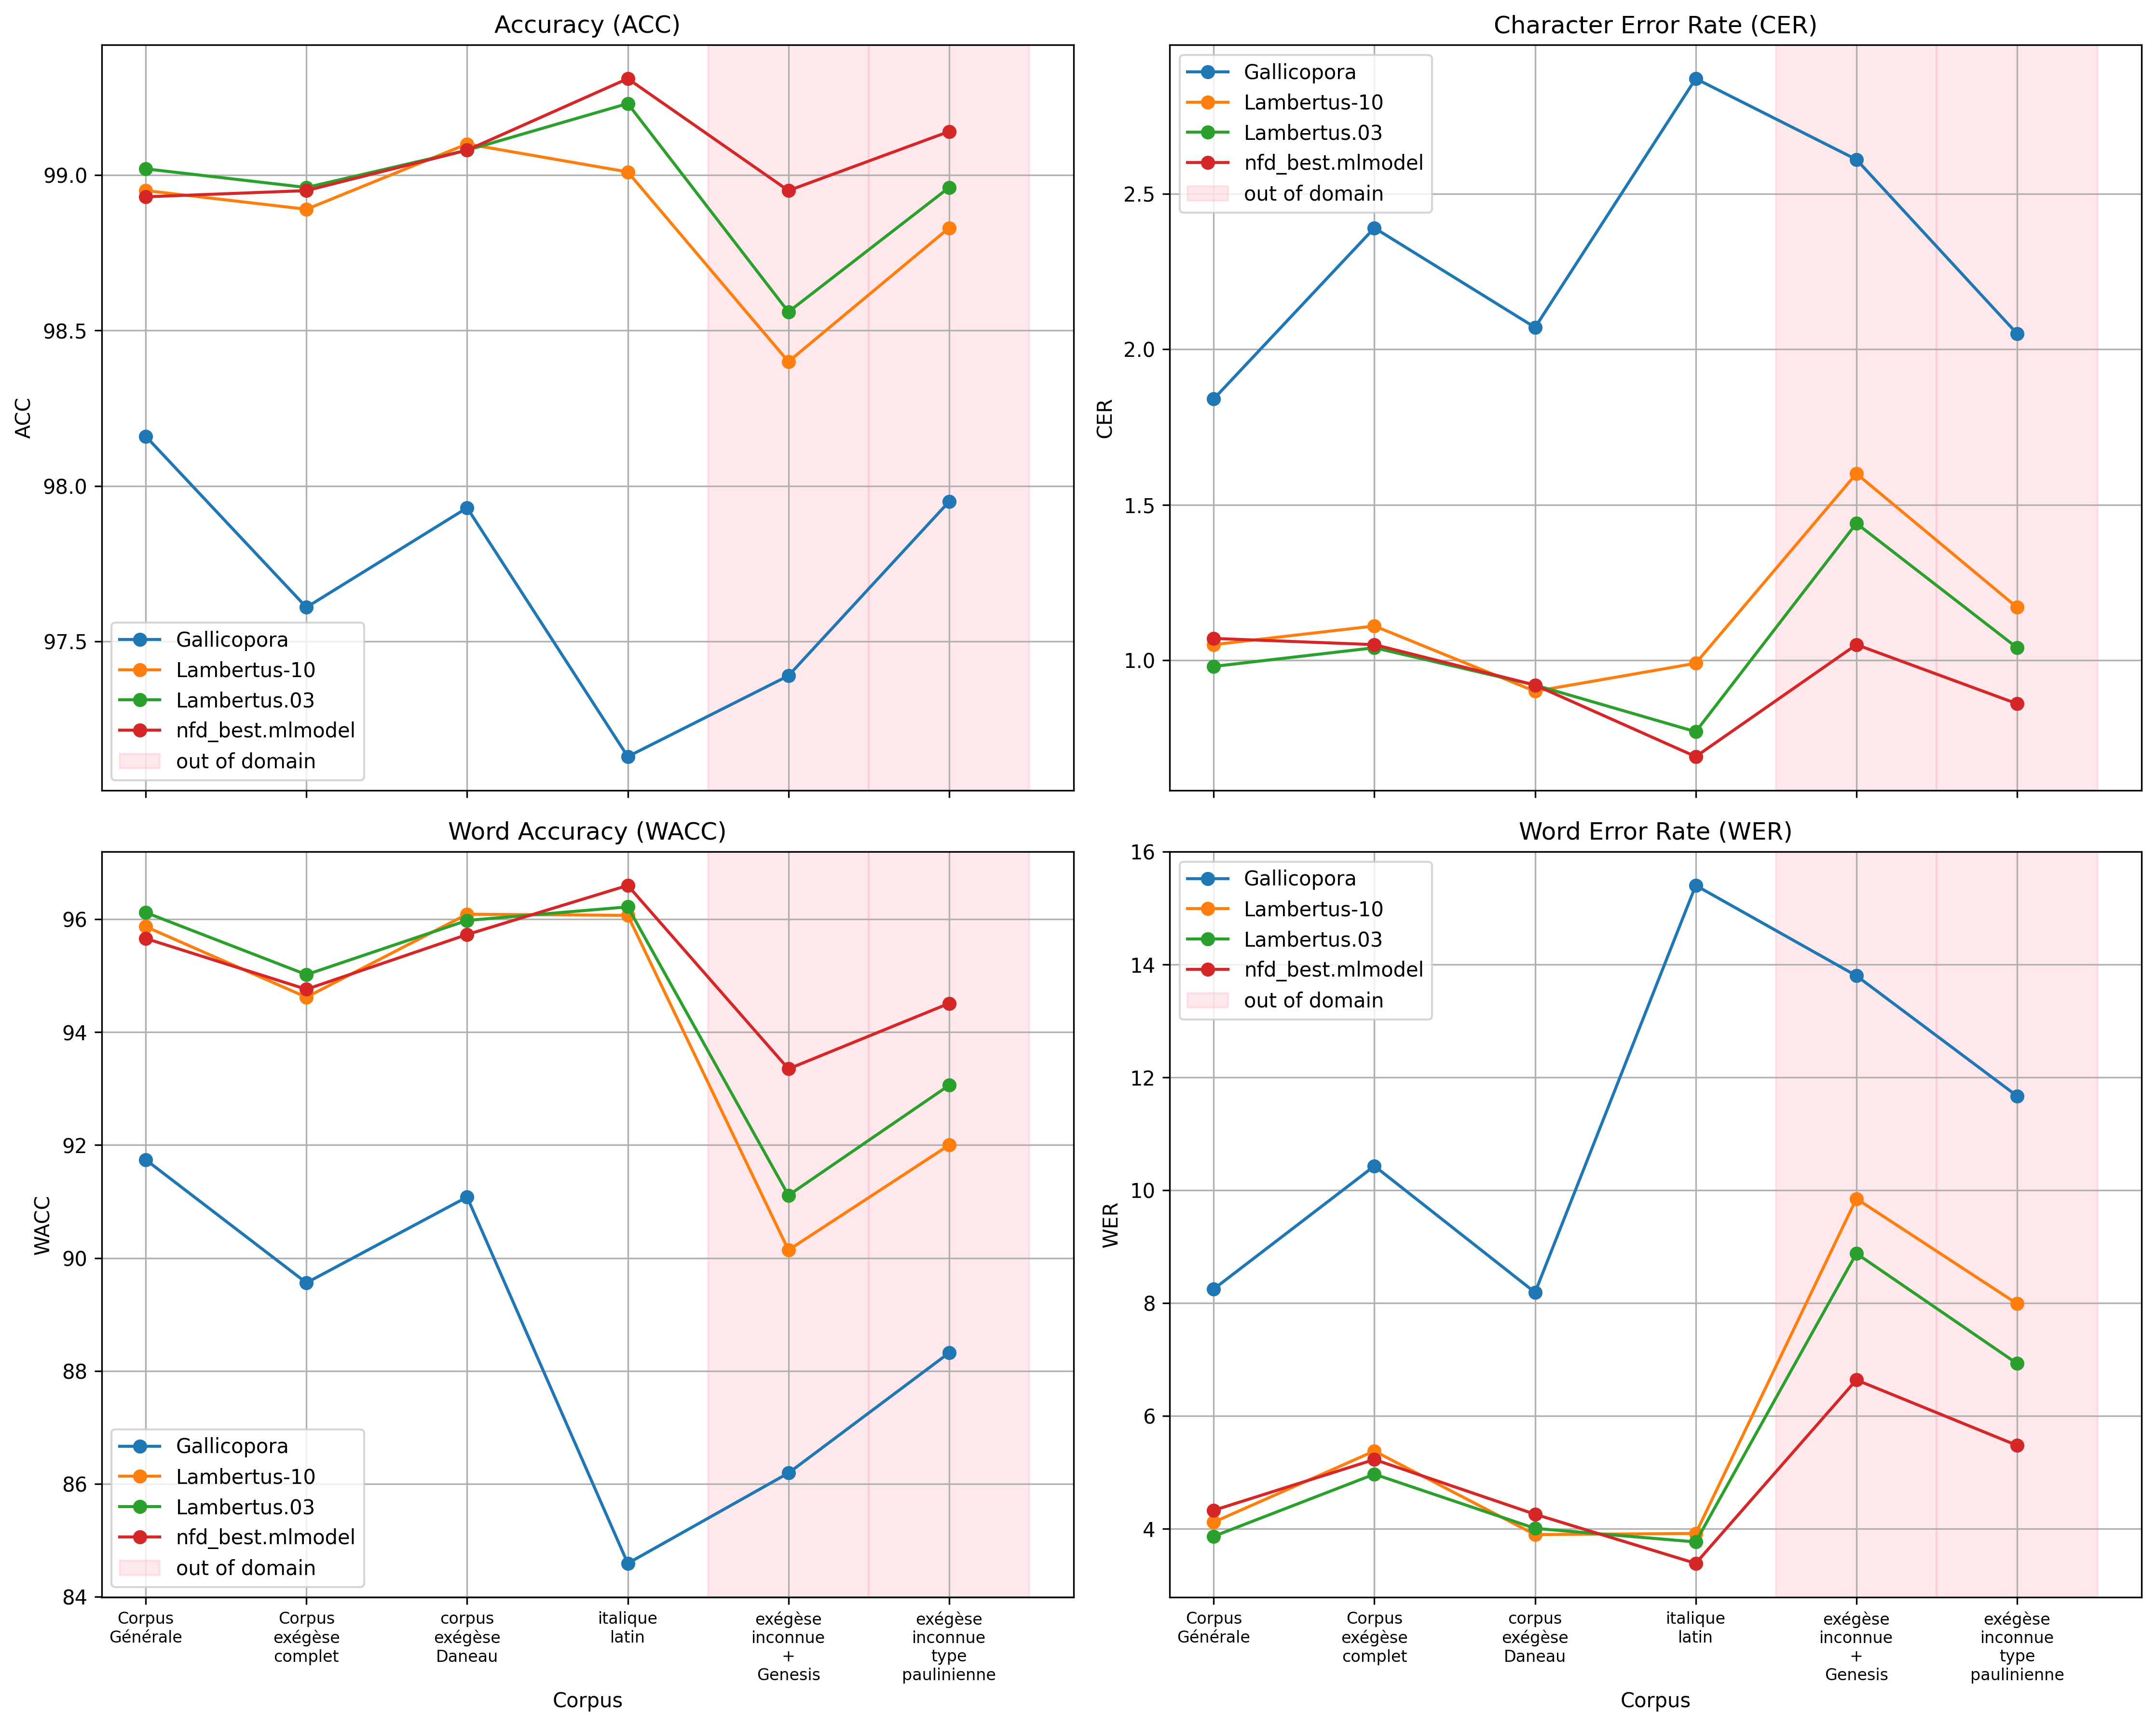
\includegraphics[width=0.9\textwidth]{comparison_metrics2.png}
    \caption{moyenne des resultats des quatre OCR.}
    \label{fig:large_graphic2}
\end{figure*}
\clearpage

\section{Lemmatisation}

Prendre 200 mots de chacun des échnatillons d'OCR.


décrire la composition du corpus 
- à timothé de lambert chap 5
- Paul autres commentaires 
- deux imprimé d'un autre texte biblique
 dans le tableau on va vers des données de plus en plus hétérogène, le but étant de tester les limites de l'OCR et du modèle de topic modelling. En permettant un teste à la fois sur le corpus interne ici les commentaires pauliniens du XVIe siècle, mais également comparaison entre le corpus interne et le corpus externe avec la aussi une gradation dans le niveau d'hétérogénité des données. Tout d'abord on se concentre sur des textes commentaire biblique mais de textes différents assez éloigné sémantiquement. Puis en faisant une comparaison avec de la poésie qui implique un autre style d'esthétique littéraire. Dans le cadre de la construction du modèle de langue, teste sur Nicolas de Lyre. Le choix d'utiliser le même corpus pour la lemmatisation et pour l'OCR comme ça on utilise le lemmatisaeur pour corriger les données...? (à vérifier) 

 

\textbf{le facteur temps}//
combien de mot par page en combien de temps 

\textbf{les limites des outils} 

Le facteur erreur dans la combinaison automatique ocr-lemmatisation
le terme ecclesia, la séparation est rarement signifié par un tiret dans l'imprimer, donc pas de signe transcrit dans l'OCR donc des erreurs dans le programme de lemmatisation 
ecc lesia// ec clesia. Du coup normaliser le terme avant. (exemple : ocr\_fail\_2012889.png)
les transition d'une page à l'autre manque également de tiret 
ou epistola
\clearpage

\FloatBarrier

\begin{figure*}[t]
\section{Pipeline pour l'édition numérique}
    \centering
    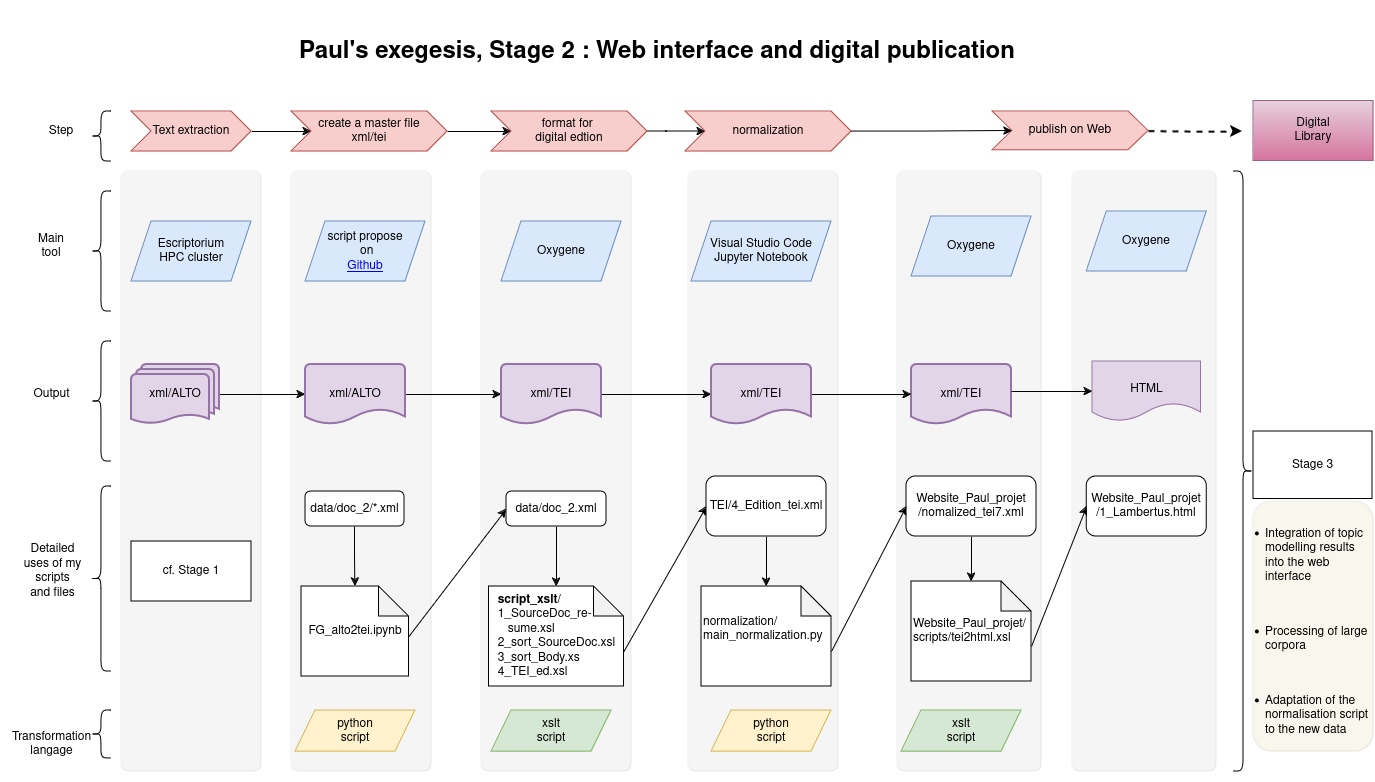
\includegraphics[width=\textwidth]{Paul_Pipeline.png}
    \caption{\href{https://github.com/FourbeFlo/PipeLine-for-Web-interface}{schéma de la pipeline d'édition digitale }}
    \label{fig:large_graphic3}
\end{figure*}

\FloatBarrier
\section{Discussion}

Ce que l'on en comprend
Est-ce pertinent de faire ça
Au vue de l'expérience, le choix premier de lemmatiser sur un texte encore abrégé ne me paraît plus pertinent. Le script de normalisation en python est beaucoup facile a mettre en place que ce que j'avais prévu. L'amélioration est également du a de mes propres compétences en compréhension de langage informatique. Ainsi à l'époque où la décision a été prise de lemmatiser directement le texte abrégé, j'aurai été incapable de créer un tel script.   

\subsubsection{points à améliorer pour l'OCR}
-contrainte temporelle, créer un corpus de toute piece = long donc reprendre des corpus existants donc choix structurelle conditionnées par de données préexistante. Dans un monde idéale, il faudrait plus de donnée de txt exegétique pour améliore la pertinence de l'ocr sur certaine abréviation => pour la suite
=> grec aussi, l'hebreux dans une moindre mesure car peut présent dans le corpus paulinien => comparaison avec la lg de base du txt paul, si par exemple on travaillait sur la Génèse. 


\FloatBarrier
\section{ Réflexions préliminaires pour le développement futur du projet }
Arrivé au terme de l'expérience, on peut désormais examiner les suites possible du projets tout en s'appuyant sur les travaux menés au cours de l'année passée.
\begin{itemize}[label=$\bullet$]
    \item élargissement du corpus de 1 à 100
\end{itemize}
Maintenant que la chaîne de traitement des données est mise en place, l'enjeu est d'examiner un très grand nombre de texte, afin de pouvoir bénéficier pleinement de l'approche computationnelle du big data. L'étape suivante du projet et donc nécessaire l'établissement d'un large corpus. L'établissement d'un corpus large suppose également un protocole de nomage défini permettant de retrouver chacun des livres traités.   
\begin{itemize}[label=$\bullet$]
    \item amélioration du modèle de langue avec l'insertion de nouvelles données
\end{itemize}
L'entrée de nouvelle quantité de mots permettra l'amélioration du modèle de langue. 
Il faut un plan de lemmatisation pour assurer une anontation régulière des données, au fur et à mesure de l'élargissement du corpus. Au vue du temps précédemment investi, il faut consacrer. La lemmatisation ne sera pas nécessaire sur la masse globale du coprus. Un choix, serait de faire le l'exercice de  lemmatisation uniquement sur les textes choisis par les collaborateurs. Cette augmentera particulièrement l'efficacité du modèle sur ces document pour l'analyse du topique modeling.   
\begin{itemize}[label=$\bullet$]
    \item La reconnaissance d'entités nommés
\end{itemize}
Dans le présent travail le découpage en verset qui structurera les comparaisons du topic modeling à été fait manuellement. Cette tâche devra être automatisée à l'avenir. L'expérience précédente permet tout de même de tirer une conclusion sur la direction à prendre dans cette nouvelle problématique. Il n'est pas pertinent d'essayer de l'intégrer lors de l'océrisation du document. -ajout à la main et variance dans le corpus. La solution est probablement d'intégrer ce découpage dans le document en TEI. 
-mais variance, entre le texte des versets et le textes cités dans les commentaires donc 
Une solution comme celle-ci pourrait être interessante à voir.
Solution en deux étapes:
1. travailler la reconnaissance des variables sur un doc en txt. 
https://www.wisecube.ai/blog/named-entity-recognition-ner-with-python/
ou un outil de type chatgpt.
2. une fois que les éléments sont tagger dans le txt. Les versets variants sont balisés et on peut avec un script basé sur des mots identiques en python tagger ces mêmes versets dans la tei. 
Le passage par le txt permet de travailler sur un document simplifié, notamment si une étape de tokenization est necessaire, ce qui sera certainement le cas.

\begin{itemize}[label=$\bullet$]
    \item la visulalisation des resultats dans une bibliothèque numérique
\end{itemize}
La bibliothèque numérique est l'objectif final du projet, mais on pourra la construire tout au long de son déploiement en ajoutant tour à tour les différents textes analysés. Il convient de réfléchir à l'architecture du site à grande échelle au moins à l'état de prototype pour anticiper dans la mesure du possible les problèmes lors de son déploiement. La maquette html peut ainsi servir de première ébauche .

potentiel plan pour l'année 2024-2025

\FloatBarrier
\section{Données}
Où sont mes données de'OCR et de lemmatisation

Protocole de nommages 
\clearpage
%here begin a new section

    % Entries for the entire Anthology, followed by custom entries
    
\FloatBarrier
\clearpage

\bibliography{bibliographie.bib} 

\end{document}
%%%%%%%%%%%%%%%%
cf note.tex for futher informations 